% !TeX spellcheck = en_GB
% Document setup
%\documentclass[AMdocument]{AMlatex}  % german version
\documentclass[AMdocument,optEnglish]{AMlatex}  % english version

\usepackage[english]{babel}
\usepackage[utf8]{inputenc}
\usepackage[affil-it]{authblk} % Affiliation of the author
\usepackage{amsmath}
\usepackage{bm} % Bold symbols in math mode
\usepackage{graphicx}
\usepackage{listings} % Code insertion
\usepackage{siunitx} % SI units
\sisetup{output-exponent-marker=\ensuremath{\mathrm{e}}}
\usepackage{booktabs} % For professional looking tables
\usepackage{multirow}
\usepackage{multicol}
\usepackage{longtable}
\usepackage{tabularx}
\usepackage{makecell}

\providecommand{\e}[1]{\ensuremath{\times 10^{#1}}}  % Scientific notation

% Set paths
\graphicspath{{./figs/}}
%\addbibresource{./_aux/literature.bib}

\begin{document}
	
\AMTitlePageDefault{Dynamic Response of a 3D Structure}{Project, Structural Dynamics (MW 2136) - SS17}{Pablo Rodríguez Robles, Matr.-Nr. 03685205}%  
%\AMTitlePageDefault{Title}{Subtitle}{Author}%  

\begin{abstract}
	In this work, a simple Finite Element code is used to model a hangar structure (see Appendix \ref{sec:hangar-description}). Once this model is set up and tested, the dynamic response of the structure is studied. This study is further divided in two parts: First, the free vibration response of the system is analysed and eigenmodes and eigenfrequencies are computed by means of the Power Iteration method with Orthogonal Deflation. Secondly, the transient response of the structure is computed using a time-integration approach with the help of implicit and explicit Newmark schemes.
\end{abstract}

\tableofcontents

\section{Beam and Bar Finite Element Model}
\label{sec:model}

\subsection{Building the Finite Element Model}

The studied structure is a hangar modelled using different bar and beam elements in a Finite Element code. After defining each of the nodes of the hangar's geometry, the finite elements are created for different materials joining these nodes. Some boundary conditions, i.e. fixations at the structure's foundation, are imposed. For a complete description of the problem's geometry consult the Appendix \ref{sec:hangar-description}.

After studying the code and the hangar representation, it was decided to add some additional bar elements to the hangar (only for this section) and observe how the structure is stiffened, leading to an increase of its eigenfrequencies (code snippet of this implementation in Appendix \ref{sec:app-addtional-bars}). As it can be seen in Figure \ref{fig:new_bars}, four new bar elements were added to the structure in the modes 1, 21, 30, 31, 101, 121, 130 and 131. Keeping everything the same (i.e. boundary conditions and rest of the elements) a free vibration test using the code included was conducted to observe how the hangar stiffness changed, see Table \ref{table:new_bars_frew}. The introduction of the new reinforcement elements increases the eigenfrequencies of the structure, which means that its stiffness is also increased. The new elements act as additional constraints between the degrees of freedom of the nodes, thus stiffening the system.

\begin{figure}[ht] 
	\centering
	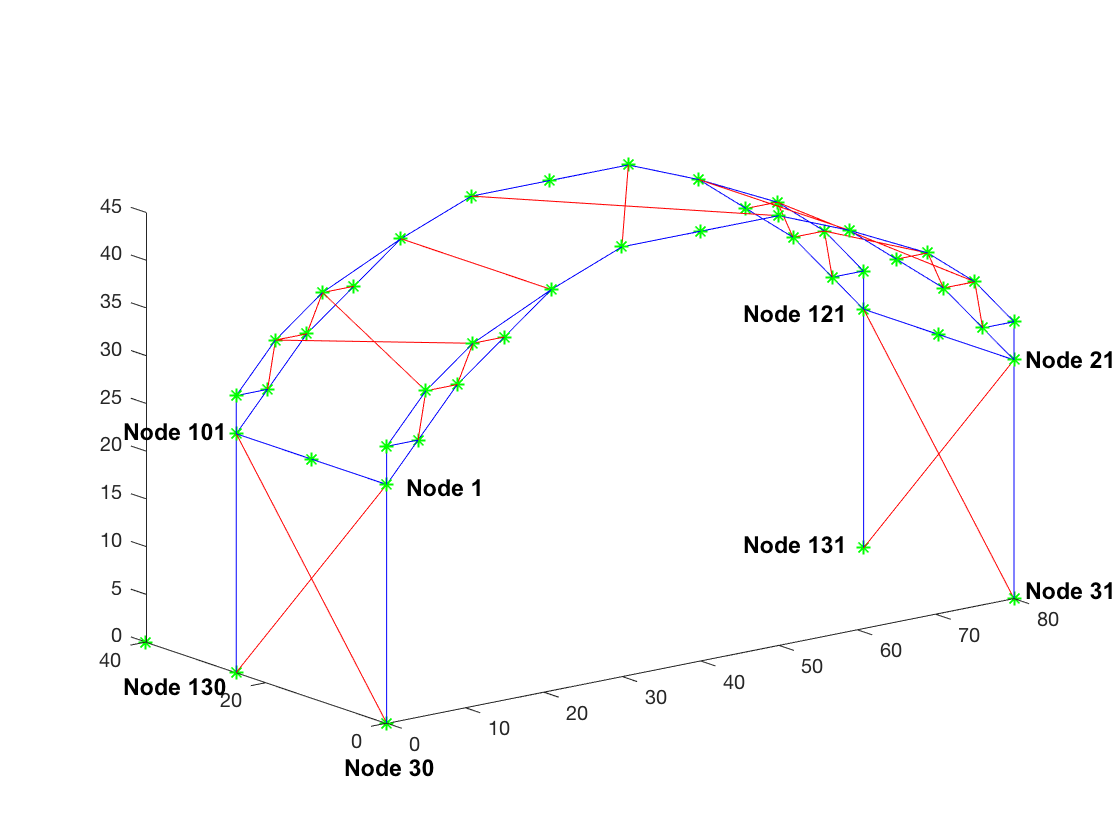
\includegraphics[width=0.6\textwidth]{additional_cross_bars} 
	\caption{New cross bars added to stiffen the structure.}
	\label{fig:new_bars}
\end{figure}

\begin{table}[]
	\centering
	\begin{tabular}{lcc}
		\toprule
		& Initial structure & Structure with new cross bars \\
		\midrule
		First eigenfrequency (\SI{}{\hertz})  & 0.2272            & 0.2616                        \\
		Second eigenfrequency (\SI{}{\hertz}) & 0.2628            & 0.2630                        \\
		Third eigenfrequency (\SI{}{\hertz})  & 0.3832            & 0.5390                        \\
		Fourth eigenfrequency (\SI{}{\hertz}) & 0.4651            & 0.5410 \\      
		\bottomrule                 
	\end{tabular}
	\caption{First four eigenfrequencies of the original and modified structure.}
	\label{table:new_bars_frew}
\end{table}

\subsection{Checking the Model}

It is possible to analyse the correct model implementation checking the rigid body modes of the structure. To do this, it is necessary to remove all the boundary conditions fixing some of the modes.

First we check that for a rigid body translation mode the model generates no force. For this purpose, the stiffness matrix $\bm{K}$ for the non-constrained system is used, i.e. the matrix $\bm{K}$ provided by the code before applying the boundary conditions. It must be satisfy

\begin{equation}
	\bm{K} \bm{u}_{trans} = \bm{0}
\end{equation}

where $\bm{u}_{trans}$ is a translation rigid body mode. For a model with $n$ nodes, since every of the nodes has 6 DoF (degrees of freedom), the translation vector $\bm{u}_{trans}$ is a ($6n \times 1$) vector with one of these patterns

\begin{align*}
	\bm{K} \bm{u}_{trans} = 
	\begin{bmatrix}
		1 & 0 & 0 & 0 & 0 & 0 & \ldots \ \\
	\end{bmatrix}^{T} \\
	\bm{K} \bm{u}_{trans} = 
	\begin{bmatrix}
		0 & 1 & 0 & 0 & 0 & 0 & \ldots \ \\
	\end{bmatrix}^{T} \\
	\bm{K} \bm{u}_{trans} = 
	\begin{bmatrix}
		0 & 0 & 1 & 0 & 0 & 0 & \ldots \ \\
	\end{bmatrix}^{T} 
\end{align*}

or any linear combination of them\footnote{No only rigid translations are permitted, it would also be possible to use rigid rotations. But they are much more difficult to impose and give the same information.}. When this operation is performed in a finite precision system like MATLAB, the result is not a vector containing all zeros, but containing very small values. Then, it is necessary to check if each element of the resulting array is zero up to a certain tolerance, which results to be true for the model presented. See Appendix \ref{sec:app-modelcheck} for the implementation.

In order to check the total mass of the structure a similar procedure can be applied. In this case the translation rigid body mode $\bm{u}_{trans}$ is limited to an unit amplitude. This is because we want to apply an unit acceleration of the structure, for a unit acceleration the inertial force produced is equal to the mass (Newton's second law). Then, the translation vector $\bm{u}_{trans}$ is a ($6n \times 1$) vector with one of these three patterns

\begin{align*}
	\bm{K} \bm{u}_{trans} = 
	\begin{bmatrix}
		1 & 0 & 0 & 0 & 0 & 0 & \ldots \ \\
	\end{bmatrix}^{T} \\
	\bm{K} \bm{u}_{trans} = 
	\begin{bmatrix}
		0 & 1 & 0 & 0 & 0 & 0 & \ldots \ \\
	\end{bmatrix}^{T} \\
	\bm{K} \bm{u}_{trans} = 
	\begin{bmatrix}
		0 & 0 & 1 & 0 & 0 & 0 & \ldots \ \\
	\end{bmatrix}^{T} 
\end{align*}

Here no combination or scaling is permitted\footnote{Actually it is possible to use a combination of accelerations in the three space directions if the modulus is one. However, the case was only checked for the simple cases assumed above.}. The total mass is computed with 

\begin{equation}
	\bm{u}_{trans}^T \bm{M} \bm{u}_{trans} = m_{total}
\end{equation}

The result is \SI{15949}{\kilogram} for all the cases tried (as expected). See also Appendix \ref{sec:app-modelcheck} for the implementation.

\section{Numerical Methods for Dynamic Analysis}
\label{sec:numerical-methods}

\subsection{Free Vibration}

Here the inverse iteration technique with deflation is implemented to compute the first eigenmodes and eigenfrequencies of the presented system. This implementation is available in the Appendix \ref{sec:inverse-interation-code}. To conduct this analysis, as well as the following, all the boundary conditions fixing the base of the structure are again imposed. 

The implementation of the inverse iteration follows the scheme proposed in the lecture notes \cite{strucdyn-lecnot}, including the orthogonal deflation to eliminate the components on the previously computed eigenmodes. 

Table \ref{table:eigfreqs} shows the result of the computation of the first 10 eigenfrequencies of the structure by means of the inverse iteration with orthogonal deflation, as well as a comparison with regard to the Matlab function \verb|eig| as a difference of $\omega_{\text{inviter}} - \omega_{\text{eig}}$, for a convergence criterion of $\epsilon =$ \num{1e-7}.

\begin{table}[]
	\centering
	\begin{tabular}{ccr}
		\toprule
		Number & Eigenfrequency (\SI{}{\hertz}) & Difference w.r.t. \verb|eig| (\SI{}{\hertz})\\
		\midrule
		1.     & \num{0.227172304677848} & \num{0.054471220312102e-7}   \\
		2.     & \num{0.262763224333734} & \num{-0.080858777451454e-7}  \\
		3.     & \num{0.383225170876377} & \num{0.006938190577621e-7}   \\
		4.     & \num{0.465050647525288} & \num{-0.009548085100342e-7}  \\
		5.     & \num{0.545936718826645} & \num{0.006106022354402e-7}   \\
		6.     & \num{0.595175315500743} & \num{-0.005646566547668e-7}  \\
		7.     & \num{0.647241555567568} & \num{-0.033387831388509e-7}  \\
		8.     & \num{0.726562208273420} & \num{-0.017445920263981e-7}  \\
		9.     & \num{0.808302304799511} & \num{-0.027269725366708e-7}  \\
		10.    & \num{1.124506735794542} & \num{0.096435655017046e-7}  \\
		\bottomrule
	\end{tabular}
	\caption{Eigenfrequencies for the first 10 eigenmodes.}
	\label{table:eigfreqs}
\end{table}

When verifying the accuracy of the computations, it can be observed that it is related to the convergence criteria (see order of magnitude of the difference in Table \ref{table:eigfreqs}). It cannot be observed that the accuracy of the higher modes is deteriorating due to the application of successive deflection. 

To further investigate this behaviour, the author decided to compute up to the first 100 of eigenfrequencies and plot the absolute value of the difference between the to methods for different convergence criteria, see Figure \ref{fig:diff-tol}. It can be observed how to up to a certain convergence criterion the solution starts to be accurate w.r.t. the Matlab \verb|eig| solution, and their difference is related to the convergence criterion used (which is related to the accuracy of the solution of the inverse iteration method). But no significant deterioration can be observed for the higher frequencies in any case.

\begin{figure}[ht] 
	\centering
	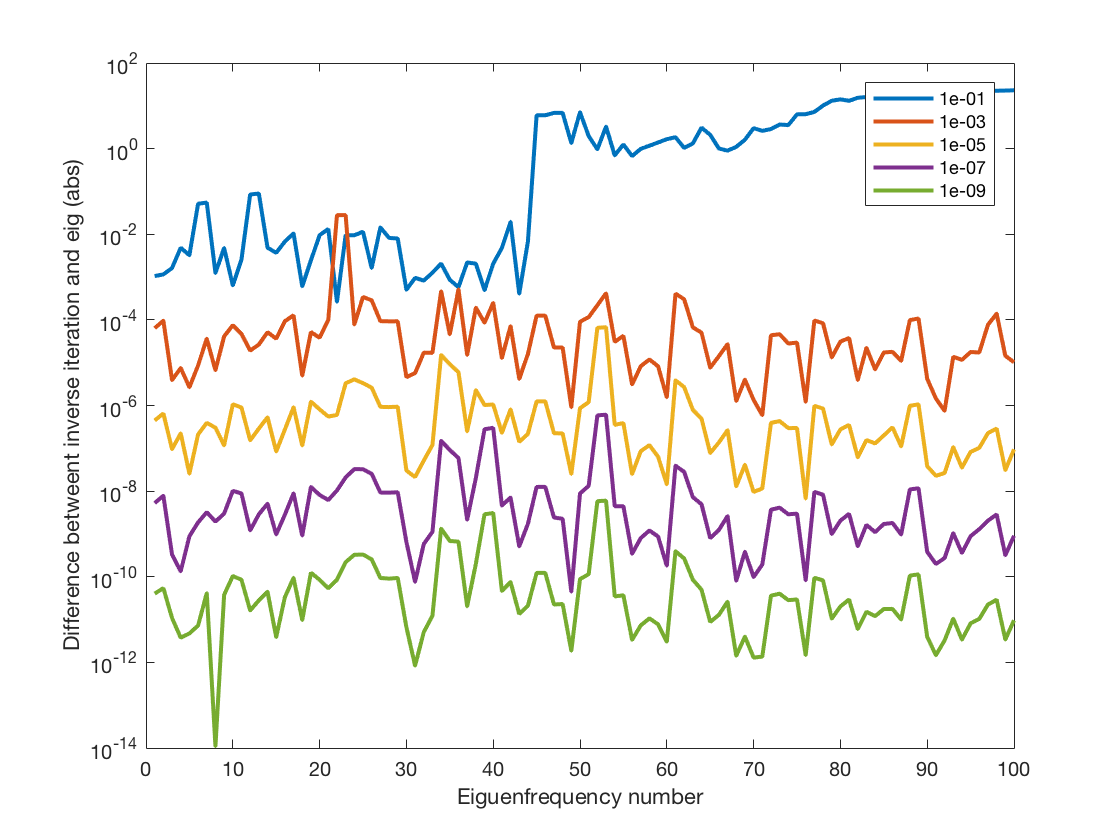
\includegraphics[width=0.6\textwidth]{differences_tol} 
	\caption{Difference between inverse iteration and eig for the first 100 eigenfrequencies and different convergence criteria.}
	\label{fig:diff-tol}
\end{figure}

From here we can conclude that the accuracy of the method does not deteriorate for higher frequencies, at least w.r.t. the result of Matlab.

It is important to note that as described in the lecture notes \cite{strucdyn-lecnot} the number of nearly converged eigenvalues is equal to half of the degrees of freedom in the model. However, the approximation obtained is an upper bound to the corresponding exact eigenvalues.

\subsection{Transient Analysis}

Here, the transient response of the hangar structure to a force applied on its frontal is computed using two different cases of the Newmark scheme. This force has the form of a triangular function, with an amplitude of \SI{100}{\newton} and a period equal to half the period of the fourth eigenfrequency (Appendix \ref{sec:force} contains the implementation of this force).

\subsubsection{Implicit Newmark Scheme}

Implicit Newmark method was implemented, using the average constant acceleration scheme (i.e. $\gamma = \frac{1}{2}$ and $\beta = \frac{1}{4}$). For such an implicit method, stability is unconditional, what means that the stability of the method is not influenced by the time step chosen. Taking this into account, it was estimated that in order to represent the higher frequencies properly, the time resolution should be smaller than the period of the highest eigenfrequency\footnote{Since the model has a finite number of degrees of freedom, it has also a finite number of eigenfrequencies, which where computed with Matlab's eig function.}. Being $\omega = \SI{355.36}{\hertz}$ its value, a time step smaller than \SI{0.0028}{\second} would represent it properly. 

For a decreasing time step the solution (see Figure \ref{fig:convergence}) starts converging when using a time step of the order \num{1e-3}, which is consistent with the assumption of a time step smaller than the period for the highest eigenfrequency.

\begin{figure}[ht] 
	\centering
	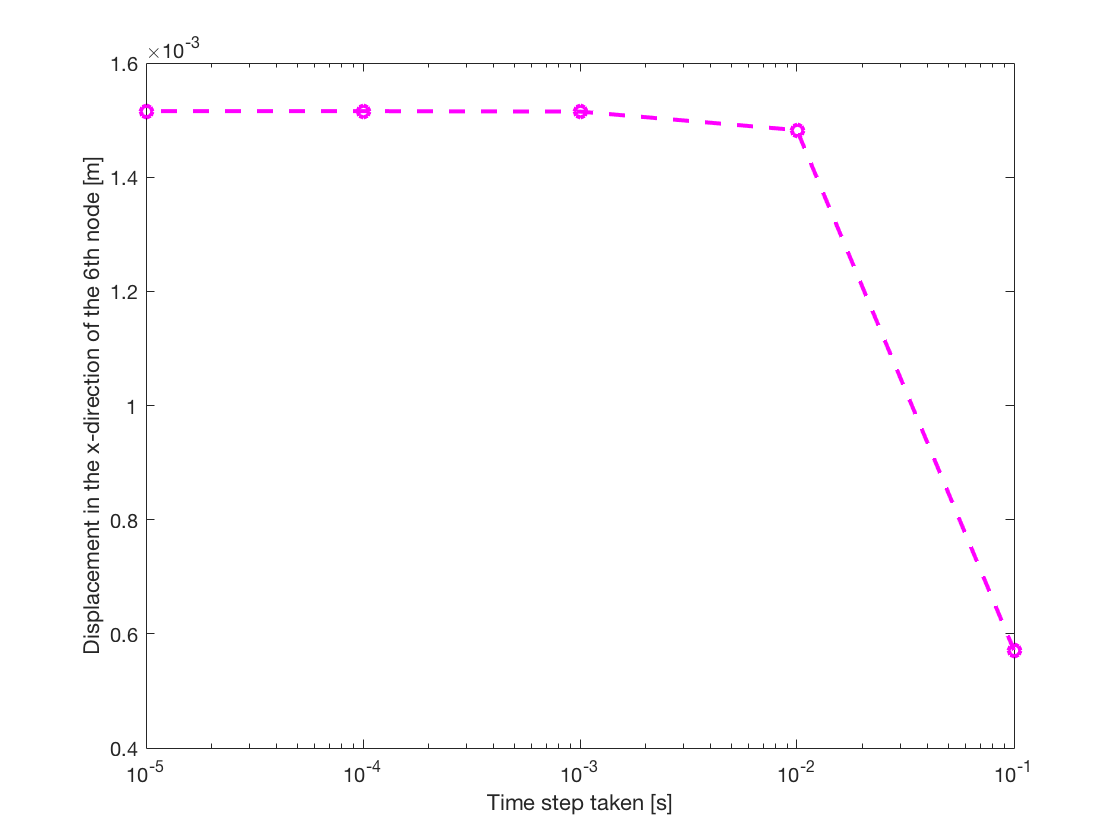
\includegraphics[width=0.6\textwidth]{convergence} 
	\caption{Convergence of the solution for displacement of node 6 in the x-direction for different time steps.}
	\label{fig:convergence}
\end{figure}

\subsubsection{Explicit Newmark Scheme}

Explicit Newmark method was implemented, using the central difference scheme (i.e. $\gamma = \frac{1}{2}$ and $\beta = 0$), which is explicit for the displacements.

The computational cost of the method was studied taking as a metric the execution time of the script containing its implementation (see Appendix \ref{sec:explicit-code}). When compared\footnote{Running on a MacBook Pro (Retina, 13-inch, Early 2015) with a 2.7 GHz Intel Core i5 processor and 8GB or RAM. Using Matlab R2016a, 64-bit (maci64) from February 11, 2016.} to the implicit scheme implemented above using a time step of \num{1e-4} for both, propagating the solution in time until 30 times the period of the excitation force, the explicit scheme took \SI{98.635}{\second} and the implicit scheme \SI{104.308}{\second}. This is not, of course, such a big difference and can be explained because the scheme implemented is not fully explicit (i.e. $\alpha$ is still not equal to zero), which means than the accelerations still need to be computed. The acceleration computation requires solving the following set of equations \cite{strucdyn-lecnot}

\begin{equation}
\begin{aligned}
\bm{S} &= \bm{M} + h \gamma \bm{C} + h^2 \beta \bm{K} \\
\bm{S} \ddot{\bm{q}}_{n+1} &= \bm{p}_{n+1} - \bm{C} \dot{\bm{q}}^\ast_{n+1} - \bm{K} \bm{q}^\ast_{n+1}
\end{aligned}
\label{eq:accelerations}
 \end{equation}
 
 Since there is no damping and $\beta = 0$, the first of the expressions above is simplified to $\bm{S} = \bm{M}$. This would be an advantage in case the system's model were using a lumped mass strategy, since the inversion of $\bm{S}$ in the second expression would be cost-free for a diagonal matrix $\bm{M}$. Since this is not the case, to compute the acceleration $\ddot{\bm{q}}_{n+1}$ is still necessary to solve a linear problem. Other difference for this scheme is that in the correction step (see Equation \ref{eq:correction}) the accelerations are not necessary to compute the new displacements, but still we need them to compute the velocities. Thus, there exist no noticeable performance improvement (i.e. the linear system of Equation \ref{eq:accelerations} must yet be solved).
 
 \begin{equation}
 \begin{aligned}
 \dot{\bm{q}}_{n+1} &= \dot{\bm{q}}^\ast_{n+1} + h \gamma \ddot{\bm{q}}_{n+1} \\
 \bm{q}_{n+1} &=  \bm{q}^\ast_{n+1} + h^2 \beta \ddot{\bm{q}}_{n+1} 
 \label{eq:correction}
\end{aligned}
\end{equation}
 
 One must conclude that the only reason to use this scheme is in presence of a lumped mass matrix (i.e. diagonal) and when a small time step is required (since the method is not unconditionally stable) because there is an special interest in the higher frequencies (impact response or wave propagation).
 
 Concerning the stability of the method, in order to satisfy the stability condition the time step $h$ must be chosen such as $\omega h \leq 2$. Where $\omega$ is the highest eigenfrequency contained in the model. Following this statement, for the system studied the time step should be 
 
$$h \leq \frac{2}{\omega}$$
$$h \leq \frac{2}{\SI{355.365}{\hertz}}$$
$$h \leq \SI{0.0056}{\second}$$

After several numerical experiments (i.e. variations of the time step and observing if the solution explodes) it was observed that the computations become unstable for a time step bigger than \SI{0.00089572}{\second}, which corresponds to a highest eigenfrequency of the order of \SI{2200}{\hertz}. The author found no explanation to this behaviour, since although it has been stated that the computation of the last half of the eigenfrequencies is not accurate, they act as an upper bound to the real eigenfrequencies of the structure. What is more, the frequency used in the definition of the stability criterion should correspond to the highest frequency that the model can achieve (which was accurately computed if compared with the Matlab solution) and not the frequency of the real physical system.
 
 When the solution (in the plot for the displacements of mode 6) of both methods is compared for the same time step of \SI{0.0001}{\second}, they seem to give the same result.
 
 \begin{figure}[ht] 
 	\centering
 	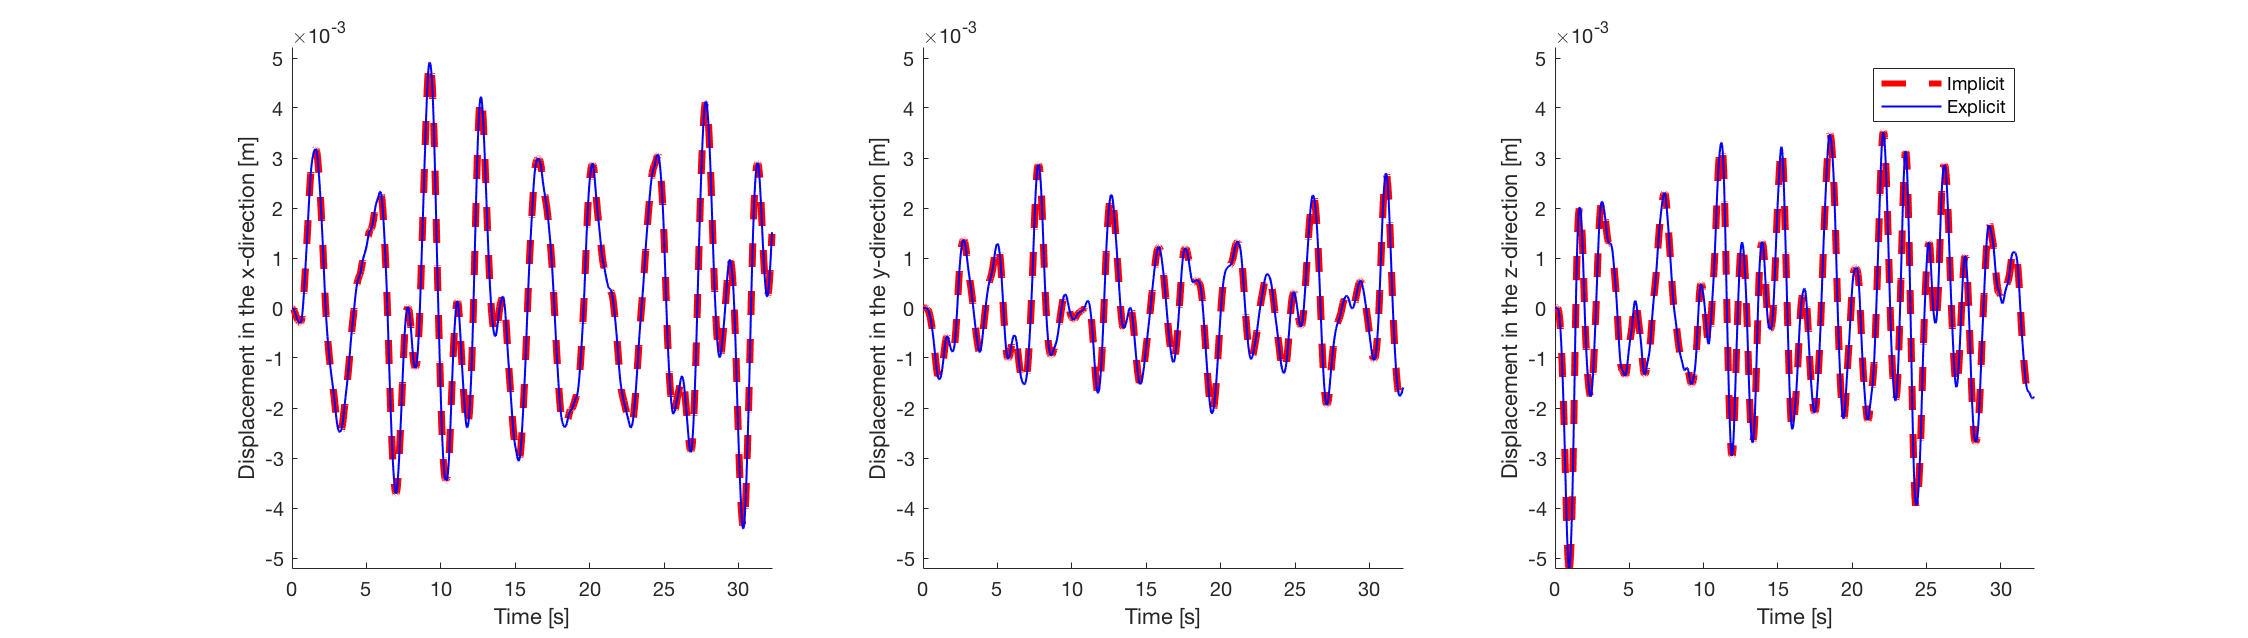
\includegraphics[width=\textwidth]{same} 
 	\caption{Comparison of implicit and explicit methods solution fo r the displacements of mode 6 with a time step of \SI{0.0001}{\second}.}
 	\label{fig:convergence}
 \end{figure}
 
\clearpage

\appendix

\section{Hangar Structure Description}
\label{sec:hangar-description}

\begin{figure}[!htb] 
	\centering
	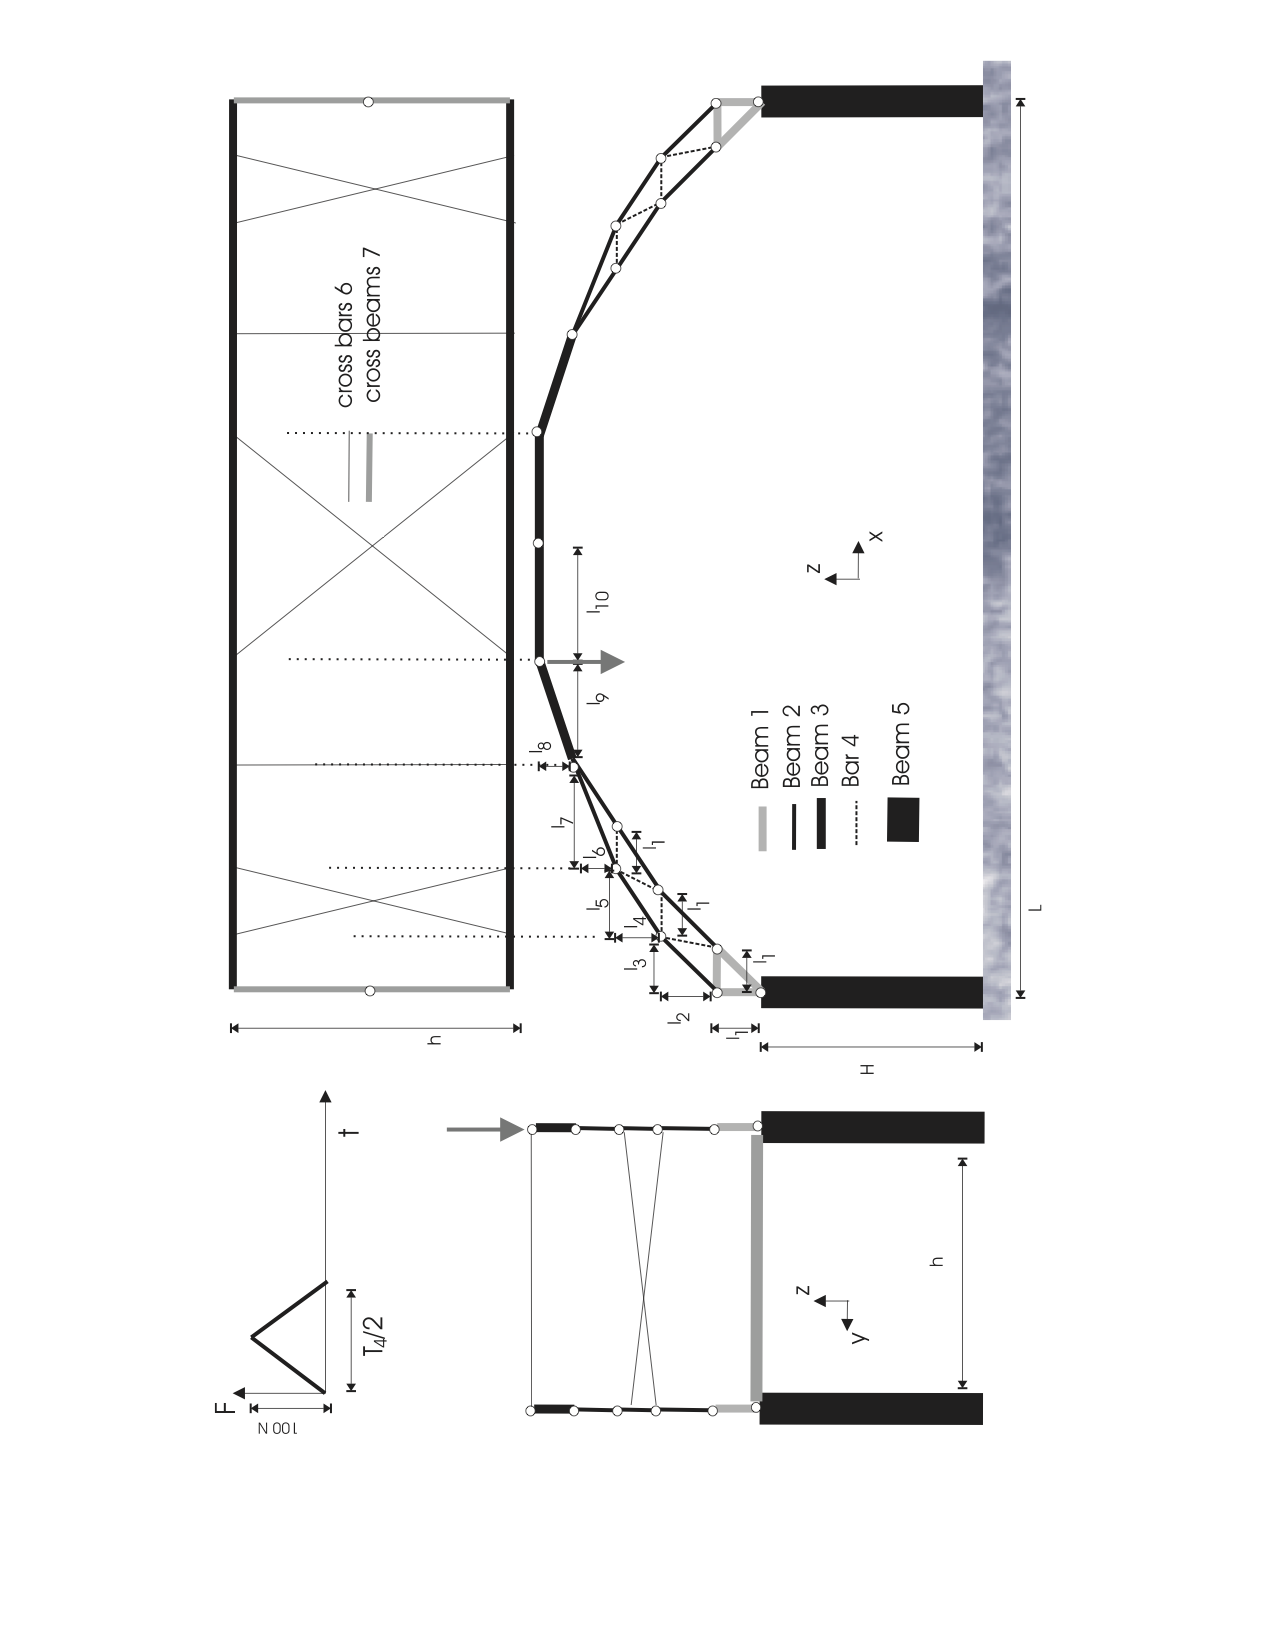
\includegraphics[width=\textwidth,height=\textheight,keepaspectratio]{hangar}
	\caption{Hangar structure.}
\end{figure}

\section{Building the Finite Element Model Code}
\label{sec:app-addtional-bars}

\begin{lstlisting}[language=Matlab]
%% Model elements

% Add additional cross bars
Elements(77,:) = [1   6       1  130  200];
Elements(78,:) = [1   6       30 101  200];
Elements(79,:) = [1   6       21 131  200];
Elements(80,:) = [1   6       31 121  200];
\end{lstlisting}

\section{Model Check Code}
\label{sec:app-modelcheck}

\begin{lstlisting}[language=Matlab]
%% Check the model: Stiffness matrix K
% Using K before applying the boundary conditions

% Get dimesions of u form K
[m, n] = size(K);

% Construct rigid body mode
u = zeros(n, 1);
u(1:6:n, 1) = 1;
u(2:6:n, 1) = 1;
u(3:6:n, 1) = 1;

% Tolerance for almost 0
eps = 1e-7;

% Ku = 0 (for almost equal, fininte precision).
% If true Ku = 0 holds
any(abs(K * u) > eps)
\end{lstlisting}

\begin{lstlisting}[language=Matlab]
%% Check the model: Total mass
% Using M before applying the boundary conditions

% Get dimesions of u form M
[m, n] = size(M);

% Construct rigid body mode
u = zeros(n, 1);
u(1:6:n, 1) = 0;
u(2:6:n, 1) = 0;
u(3:6:n, 1) = 1;

% u'Mu = m_total
% Returns 1.5949e+04 kg for all cases
u' * M * u
\end{lstlisting}

\section{Inverse Iteration Method with Orthogonal Deflation Code}
\label{sec:inverse-interation-code}

\begin{lstlisting}[language=Matlab]
%% Compute eigensolutions: Inverse Iteration Method

% Make K and M full
K = full(K);
M = full(M);

% Check K is not singular using rank
[m, n] = size(K);
if rank(K) < m 
error('K is not singular')
end

% Tolerance for convergence check using Rayleight quotients
eps = 1e-7;

% Number of eigenvalues computed
neig = 10;

% Matrix containing the orthonomalization operators.
% Inintially identity, when a new eigenmode is found
% the new operator is included using matrix multiplication:
% P = I*P1*P2*P3...Pk
P = eye(size(M));

% Preallocation of vector containing the
% eigenfrequencies of the system
omega2 = zeros(neig, 1);

% Preallocation of vector containing the
% eigenfrequencies of the system
eigmodes = zeros(m, neig);

% Althoug it is more efficient to use directly
% Matlab's backslash operator, here LU is used to
% look at the outputs.
[L,U] = lu(K);

for j=1:neig

% Arbitrary starting vector
z0 = rand(n, 1);
z = z0;

% Rayleight quotient
rayquo = (z' * K * z) ./ (z' * M * z);

% Previous Rayleight quotient
rayquo_0 = 0;

% Convergence condition,
% 1 meaning 'True'
condition = 1;

% Used to count number of iterations carried
iter = 0;

while condition

% Removes components of the already computed
% eigenmodes from the starting vector
z = P * z;

% Partial solution
y = M * z;

% New iterate z
% LUz = Lb = y, Uz = b
b = L\y;
z = U\b;

% Normalized iterate
z = z / norm(z);

% Rayleight quotient
rayquo_0 = rayquo;
rayquo = (z' * K * z) / (z' * M * z);

% Convergence condition. 
% If greater than the tolerance keep iterating
condition = abs(rayquo - rayquo_0) > eps;

iter = iter + 1;
end

% Eigenmode
x = z;

% Add normalisation operator to the rest of them
P = P * (eye(size(M)) - (x * x' * M) / (x' * M * x));

% Add computed eigenfrequency
omega2(j) = rayquo;

% Add computed eigenmode
eigmodes(:, j) = x;
end

% The threshold used as tolerance for the inverse power influences
% the difference betweeen the Matlab computations and the computations from
% the code.

% Show more decimal places
format long

omega2(1:neig);
eigenfreq_inverse = sqrt(omega2)/(2*pi)
\end{lstlisting}

\section{Transient Force Code}
\label{sec:force}

\begin{lstlisting}[language=Matlab]
function [ F ] = force( t, Ndof, locnod, dof_rem )
% Force applied on the hangar.
% Its time variation is a triangular function af total 
% length equal to half the period of the fourth eigenfrequency
% and has an amplitude of 100 N.

% Half the period of the fourth eigenfrequency
T = 0.5 * (1 / 0.4651);

if (t < 0) || (t > T)
f = 0;

elseif t < T / 2
f = 100 / (T / 2) * t;

else
f = 200 - 100 / (T / 2) * t;

end

% Ndof, number of degrees of freedom after applying boundary conditions
F = zeros(Ndof, 1);

% Force is applied vertically and pointing downwards on Node 9
loc = locnod(9, 3);

F(loc) = - f;

F = F(dof_rem);

end
\end{lstlisting}

\section{Implicit Newmark Scheme Code}
\label{sec:implicit-code}

\begin{lstlisting}[language=Matlab]
%% Transient dynamics: Implicit Newmark scheme

% Newmark scheme parameters
% (Averaged constant acceleration)
gamma = 1/2;
beta = 1/4;

% Make K and M full
K = full(K);
M = full(M);

% Dimensions of M (and K) after BCs
[m, n] = size(M);

% Half the period of the fourth eigenfrequency
T = 0.5 * (1 / 0.4651);

% Time boundaries [s]
t0 = 0;
tf = 30 * T;

% Time step [s]
step = [1e-1 1e-2 1e-3 1e-4 1e-5];
sol = zeros(length(step), 1);

for j=1:length(step)

h = step(j);

% Time [s]
time = t0:h:tf;

[~, s] = size(time);

% Vector of displacements
q_0 = zeros(m, 1);
q = zeros(m, s);
q(:, 1) = q_0;

% Vector of velocities
q_dot0 = zeros(m, 1);
q_dot = zeros(m, s);
q_dot(:, 1) = q_dot0;

% Vector of accelerations
% Case 1, initial acceleration equals zero
q_ddot0 = zeros(m, 1);
q_ddot = zeros(m, s);
q_ddot(:, 1) = q_ddot0;

% Vector of accelerations
% Case 2, compute initital acceleration
% (In this case not necessary)

% External force at time t0
% p = force(t0, Ndof, locnod, dof_rem);

% q_ddot0 = M \ (p - K * q_0)

% For a constant time step h, S does not change.
% Its factorization can be reutilized
S = M + h^2 * beta * K;
[L,U] = lu(S);


for i = 1:s-1

% Prediction
q_dotstar = q_dot(:, i) + (1 - gamma) .* h .* q_ddot(:, i);
q_star = q(:, i) + h .* q_dot(:, i) + ...
(0.5 - beta) .* h.^2 .* q_ddot(:, i);

% Acceleration
p = force(time(i+1), Ndof, locnod, dof_rem);

% LU q_ddot = L b = (p - K * q_star), U q_ddot = b
b = L \ (p - K * q_star);
q_ddot(:, i+1) = U \ b;

% Correction
q_dot(:, i+1) = q_dotstar + h .* gamma .* q_ddot(:, i+1);
q(:, i+1) = q_star + h.^2 .* beta .* q_ddot(:, i+1);

end

% Save x-direction displacement of the 6th node
sol(j) = q(31 , end);
end
\end{lstlisting}

\section{Explicit Newmark Scheme Code}
\label{sec:explicit-code}


\begin{lstlisting}[language=Matlab]
%% Transient dynamics: Explicit Newmark scheme

% Newmark scheme parameters
% (Averaged constant acceleration)
gamma = 1/2;
beta = 0;

% Make K and M full
K = full(K);
M = full(M);

% Dimensions of M (and K) after BCs
[m, n] = size(M);

% Half the period of the fourth eigenfrequency
T = 0.5 * (1 / 0.4651);

% Time boundaries [s]
t0 = 0;
tf = 30 * T;

% Time step [s]
step = [1e-4];
sol = zeros(length(step), 1);

for j=1:length(step)

h = step(j);

limit = 355.3646 * h;
if limit > 2;
disp('Unstable')
else
disp('Stable')
end

% Time [s]
time = t0:h:tf;

[~, s] = size(time);

% Vector of displacements
q_0 = zeros(m, 1);
q = zeros(m, s);
q(:, 1) = q_0;

% Vector of velocities
q_dot0 = zeros(m, 1);
q_dot = zeros(m, s);
q_dot(:, 1) = q_dot0;

% Vector of accelerations
% Case 1, initial acceleration equals zero
q_ddot0 = zeros(m, 1);
q_ddot = zeros(m, s);
q_ddot(:, 1) = q_ddot0;

% Vector of accelerations
% Case 2, compute initital acceleration
% (In this case not necessary)

% External force at time t0
% p = force(t0, Ndof, locnod, dof_rem);

% q_ddot0 = M \ (p - K * q_0)

% For a constant time step h, S does not change.
% Its factorization can be reutilized
S = M;
[L,U] = lu(S);


for i = 1:s-1

% Prediction
q_dotstar = q_dot(:, i) + (1 - gamma) .* h .* q_ddot(:, i);
q_star = q(:, i) + h .* q_dot(:, i) + ...
0.5 .* h.^2 .* q_ddot(:, i);

% Acceleration
p = force(time(i+1), Ndof, locnod, dof_rem);

% LU q_ddot = L b = (p - K * q_star), U q_ddot = b
b = L \ (p - K * q_star);
q_ddot(:, i+1) = U \ b;

% Correction
q_dot(:, i+1) = q_dotstar + h .* gamma .* q_ddot(:, i+1);
q(:, i+1) = q_star;

end

% Save x-direction displacement of the 6th node
sol(j) = q(31 , end);

end
\end{lstlisting}

\newpage

\addcontentsline{toc}{section}{References}

\bibliographystyle{ieeetr}
\bibliography{references}

\end{document}
